\documentclass{fiwthesis}

% ========
%  Pakete
% ========

\usepackage{textgreek}           % griechische Buchstaben außerhalb des Math-Mode
\usepackage{amsmath}             % zentrierte Formeln
\usepackage{amssymb}             % erweiterter Formelsatz mathem. Symbole

\usepackage{boldline}            % breitere Linien in Tabellen
\usepackage{booktabs}            % typographisch richtige Tabellen setzen
\usepackage{tabularx}            % Erweiterte Tabellendarstellung
\usepackage{multirow}            % Spalte über mehrere Zeilen oder Spalten ausdehnen
\usepackage{xltabular}           % Zeilenumbrüche in tabularx erlauben

\usepackage{graphicx}            % ermöglicht das Einbinden von Grafiken
\usepackage{subcaption}          % mehrere Bilder in einem Bild
\usepackage{pgfplots}            % Grafiken erzeugen
\usepackage{smartdiagram}        % schnelle und einfache Grafiken
\usetikzlibrary{positioning}     % bessere Ortsbezeichnung
\usetikzlibrary{shapes}          % typische Formen wie Rechtecke, Ellipsen usw. einfach zeichnen
\usetikzlibrary{intersections}   % Schnittpunkt von Geraden adressieren
\usetikzlibrary{angles, quotes}  % einfacheres Zeichnen von Winkeln
\usetikzlibrary{                 % Symbole für Schaltpläne
  circuits.logic.US,
  circuits.logic.IEC,
  circuits.logic.CDH,
  circuits.ee.IEC
}

\usepackage{lipsum}

% ===========
%  Metadaten
% ===========

\thesis{Projektseminar}
\title{Entwicklung eines EEG Signalgenerators}
\author{Johannes}
\matrnr{123456}
\bdate{08.11.1848}
\bcity{Wismar}
\supervisor{Prof.~Dr.~Simanski}
%\secsupervisor{}
\keywords{Logik, Mathematik}

% Metadaten in die PDF-Datei schreiben
\makepdfmetadata

% ===============
%  Präambel
% ===============

% PGF Kompatibilitätseinstellung
\pgfplotsset{width=0.95\textwidth,compat=newest}

% % Bibliographie einbinden
\bibliography{quellen}

% Glossar einbinden
\newglossaryentry{nosql}{%
  name = {NoSQL},
  description = {Kurzform für ,,Not Only SQL``; Überbegriff für Datenbanken, die das Konzept relationaler Datenbanken erweitern}
}

\newdualentry{dac}% label
{DAC}% short form
{Digital-Analog-Converter}% long form
{Ein Digital-Analog-Converter (deutsch: Digital-Analog-Wandler) ist ein Chip, der aus einem Digitalem Signal eine Analoge Spannung erzeugt.}% description

% Abkürzungen einbinden
%\gls{}         normal zu nutzen (erstes Mal: 'lange Form (kurze Form)'), danach nur 'kurze Form'
%\glspl{}       wie \gls{} nur als Plural
%\acrfull{qrc}  gibt volle Form ('lange Form (kurze Form)') egal wo
%\acrlong{qrc}  gibt lange Form ('lange Form') egal wo
%
%\newacronym{tag}{short}{long}
\newacronym{lamp}{LAMP}{Linux, Apache, MySQL, PHP}
\newacronym{qrc}{QR-Code}{Quick Response Code}


% Symbole einbinden
\newglossaryentry{symb:phi}{
  name=$\phi$,
  description={Ein beliebiger Winkel},
  sort=symbolphi, type=symbolslist
}

\newglossaryentry{symb:e}{
  name=$e$,
  description={Die Eulersche Zahl},
  sort=symbole, type=symbolslist
}


% Glossar- und Abkürzungsverzeichniserstellung
\makeglossaries{}

% Index erzeugen
\makeindex[
  intoc=true,
  title=Index,
  columns=2]{}
\indexsetup{headers={\indexname}{\indexname}}

% ===============
%  Eigene Makros
% ===============

\newcommand*{\code}[1]{\texttt{#1}}

% ===============
%  Beginn Thesis
% ===============

\begin{document}

% ============
%  "Vorspann"
% ============

% Titelseite
\maketitle

% Aufgabenstellung
% \maketask{\textbf{\underline{ACHTUNG!}}
\par
Die ausgehändigte Originalaufgabenstellung (und bei jeder Kopie
die entsprechenden Kopie) wird ohne Seitenzahlangabe
eingebunden. Bei deutschsprachigen Aufgabenstellungen wird
der Titel in englischer Sprache wiederholt.
\par
Für die digitale Fassung der Arbeit ist eine Schilderung der Aufgabenstellung aber durchaus sinnvoll und kann an dieser Stelle verfasst werden.
}

% Abstract
\makeabstract{
  Maximal eine halbe Seite.
}{
  English Version.
}

% Inhaltsverzeichnis (Schalter `compact' sorgt für einfachen Zeilenabstand)
\maketoc[compact]

% ==========
%  Textteil
% ==========

% Einleitung
\input{kapitel/Einleitung}

% weitere Kapitel hier jeweils einzeln einbinden
\section{Zielsetzung und Anforderungen}

Ziel dieses Kapitels ist die Darstellung der technischen Anforderungen und der strukturellen Umsetzung der entwickelten Platine. Die Schaltung dient als Demonstrations- und Lehrgerät zur Veranschaulichung synthetisch erzeugter EEG-Signale im schulischen oder hochschulischen Unterricht.
Kernziel der Platine ist die Erzeugung und analoge Ausgabe von EEG-Signalen über vier getrennte Kanäle. Die Parametrierung der Signale erfolgt über eine browserbasierte Benutzeroberfläche, die ohne zusätzliche Softwareinstallation genutzt werden kann. Die gesamte Steuerung und Ausgabe wird durch einen Mikrocontroller übernommen, der sowohl die Signalverarbeitung als auch die Bereitstellung der Weboberfläche realisiert.
Zur Sicherstellung einer realistischen Signalform und zur Rauschunterdrückung kommen ein hochauflösender Digital-Analog-Wandler sowie nachgeschaltete analoge Tiefpassfilter zum Einsatz. Zusätzlich wird das Ausgangssignal über einen Spannungsteiler skaliert, um typische EEG-Signalpegel im Mikrovoltbereich darzustellen.
Die folgenden Abschnitte beschreiben die eingesetzten Komponenten, ihre Auswahlkriterien und die Umsetzung auf der entwickelten Platine.


\chapter{Platine}

\section{Komponentenübersicht}

Für die Umsetzung der Platine wurden gezielt Bauteile ausgewählt, die eine zuverlässige Signalverarbeitung sowie eine einfache Integration in ein schulisches Umfeld ermöglichen. Die wichtigsten Hardwarekomponenten sind:

\begin{itemize}
  \item \textbf{Mikrocontroller:} ESP32-S3 16R8 – steuert die gesamte Signalverarbeitung, erzeugt die digitalen Datenmuster und stellt die Weboberfläche über WLAN bereit.
  \item \textbf{Digital-Analog-Wandler (DAC):} DAC8412FPZ – ermöglicht die hochauflösende, analoge Ausgabe der zuvor digital berechneten EEG-Signale auf vier unabhängigen Kanälen.
  \item \textbf{Operationsverstärker:} TL071CDR – dient als aktiver Tiefpassfilter (1. Ordnung) mit einer Verstärkung von 1 zur Glättung der analogen Ausgangssignale.
  \item \textbf{Spannungsversorgung:}
  \begin{itemize}
    \item \textbf{NCV1117DT50:} Linearregler zur Bereitstellung einer stabilisierten 5-V-Spannung für den DAC und nachgeschaltete Stufen.
    \item \textbf{USB-C-Buchse:} Dient sowohl der Stromversorgung als auch der optionalen Datenverbindung während der Entwicklung.
  \end{itemize}
\end{itemize}


\subsection{Hardwarekonzept}

Der Mikrocontroller ESP32-S3 16R8 bildet das zentrale Steuerelement der Platine. Er verfügt über zwei Prozessorkerne, wodurch sich die Verarbeitung von Signalmustern und die Bereitstellung der Weboberfläche auf getrennte Kerne verteilen lassen. Mit 16\,MB integriertem Flash-Speicher bietet er zudem ausreichend Kapazität zur Ablage von Firmware, Webdateien und Nutzdaten.

Für die analoge Signalausgabe wird der Digital-Analog-Wandler DAC8412FPZ von Analog Devices eingesetzt. Dieser 12-Bit-DAC besitzt vier voneinander unabhängige Ausgänge und wird über eine parallele 16-Bit-Schnittstelle angesteuert. Die Ansteuerung ermöglicht eine hohe Datenrate und unterstützt somit eine nahezu echtzeitfähige Signalübertragung.

Zur Nachbearbeitung der DAC-Ausgabe wird ein aktiver Tiefpassfilter auf Basis des Operationsverstärkers TL071CDR verwendet. Dieser glättet die Treppenspannung des DACs und unterdrückt hochfrequentes Rauschen, um ein möglichst sauberes analoges Ausgangssignal zu erzeugen.

Die Spannungsversorgung der Komponenten wird durch mehrere Regler bereitgestellt: Ein Linearregler (LDO) liefert 5\,V für den DAC und nachgeschaltete Stufen, ein weiterer LDO stellt 3{,}3\,V für den Mikrocontroller bereit. Zusätzlich erzeugt ein invertierender DC/DC-Wandler die negative Versorgungsspannung, sodass der DAC und die Operationsverstärker symmetrisch mit \(\pm5\,\text{V}\) betrieben werden können.

\clearpage

\section{Schaltungsdesign}
\subsection{Gesamtüberblick}
\begin{figure}[H]
    \centering
    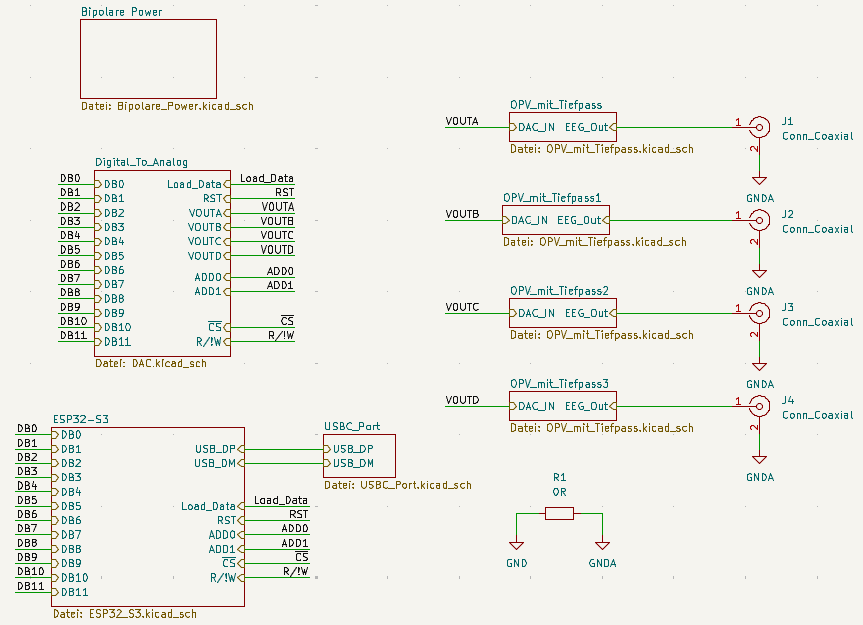
\includegraphics[width=0.8\textwidth]{bilder/Platine_gesamt.png}
    \caption{Gesamtübersicht der Platine}
    \label{fig:gesamtuebersicht}
\end{figure}
Die Schaltung ist modular aufgebaut und in mehrere funktionale Blöcke gegliedert, die jeweils klar definierte Aufgabenbereiche abdecken:

\begin{itemize}
    \item \textbf{Mikrocontroller-Block:} Beinhaltet den ESP32-S3 16R8, der die gesamte Steuerlogik sowie die Webschnittstelle übernimmt.
    \item \textbf{DAC-Block:} Umfasst den DAC8412FPZ zur Umwandlung der digitalen Signalmuster in analoge Ausgangssignale.
    \item \textbf{Operationsverstärker-Block:} Realisiert die analoge Filterung der DAC-Ausgänge mittels aktiver Tiefpassfilter.
    \item \textbf{Spannungsversorgungsblock:} Stellt alle benötigten Spannungen bereit (5 V, ±5 V, 3{,}3 V) inklusive Referenzspannungen.
    \item \textbf{USB-Block:} Dient als Schnittstelle zur Stromversorgung über USB-C.
\end{itemize}




\subsection{Mikrocontroller-Block}
\begin{figure}[H]
    \centering
    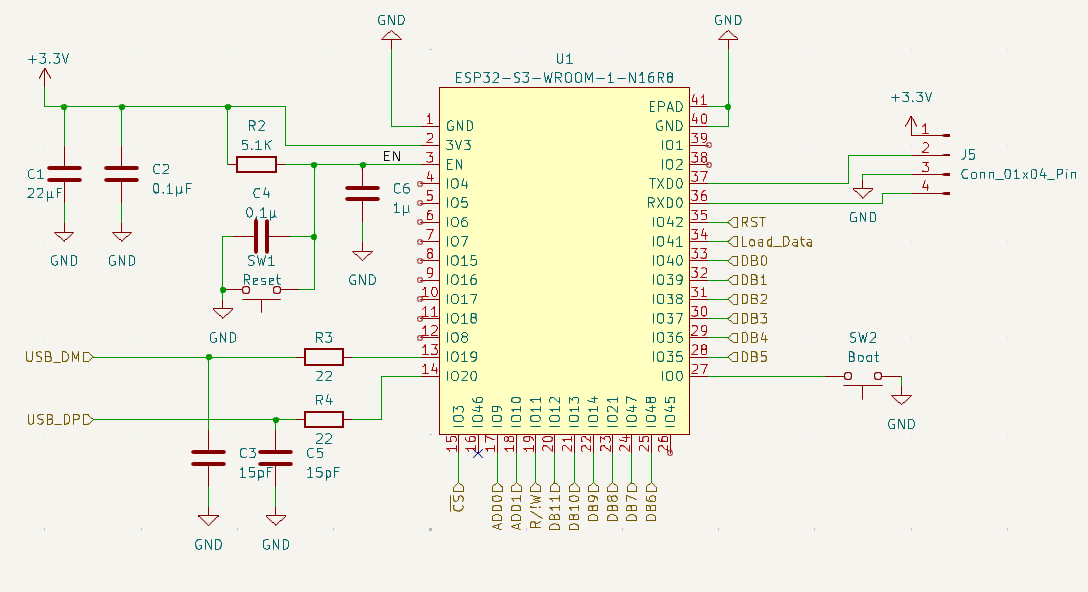
\includegraphics[width=0.8\textwidth]{bilder/Mikrocontroller_Block.png}
    \caption{Mikrocontroller-Block der Platine}
    \label{fig:mikrocontroller_block}
\end{figure}

Der Mikrocontroller-Block bildet die zentrale Steuereinheit der Platine. Herzstück ist der ESP32-S3 16R8, der sowohl die Erzeugung der digitalen EEG-Signalmuster als auch die Bereitstellung der Weboberfläche übernimmt. Die Kommunikation mit dem DAC erfolgt über eine 16-Bit-Parallelschnittstelle, wodurch eine hohe Übertragungsrate und geringe Latenz erreicht werden.
Die Programmierung des Mikrocontrollers erfolgt in C++ unter Verwendung der Arduino-Entwicklungsumgebung, ergänzt durch das Build-System PlatformIO. Neben der Echtzeitsteuerung der Signalausgabe ist der ESP32 auch für das Dateihandling sowie die Konfigurationslogik zuständig.

\subsection{DAC-Block}
\begin{figure}[H]
    \centering
    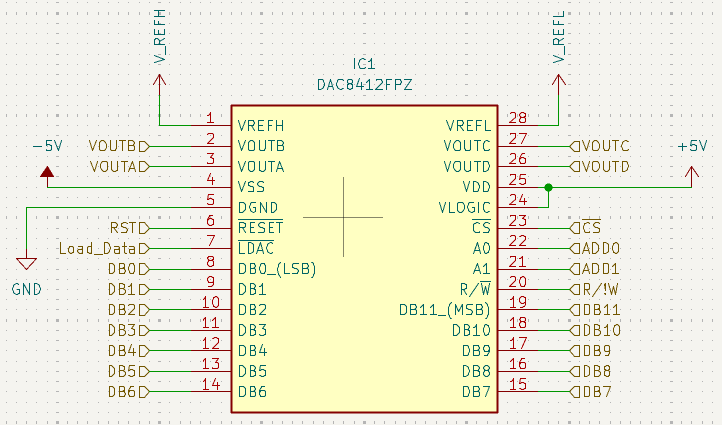
\includegraphics[width=0.8\textwidth]{bilder/DAC.png}
    \caption{DAC-Block der Platine}
    \label{fig:dac_block}
\end{figure}

Der DAC-Block umfasst den Digital-Analog-Wandler DAC8412FPZ von Analog Devices. Dieser 12-Bit-DAC ist für die Umwandlung der vom Mikrocontroller erzeugten digitalen Signalmuster in analoge Spannungen verantwortlich. 
Die Ansteuerung erfolgt über eine parallele 16-Bit-Schnittstelle, bei der alle relevanten Datenbits gleichzeitig übertragen werden. Diese Übertragungsart ermöglicht eine hohe Datentransferrate bei gleichzeitig geringer Latenz und eignet sich daher besonders für zeitkritische Anwendungen wie die synchrone Ausgabe mehrerer Kanäle.
Der DAC8412FPZ stellt vier voneinander unabhängige Ausgänge bereit. Jeder dieser Kanäle kann ein separates, kontinuierliches EEG-Signal ausgeben. Die Zuordnung der Signaldaten zu den Ausgängen erfolgt über die Softwarelogik im Mikrocontroller. Die resultierenden Spannungen an den DAC-Ausgängen werden anschließend in den analogen Nachbearbeitungsblock überführt.


\subsection{Operationsverstärker-Block}

\begin{figure}[H]
    \centering
    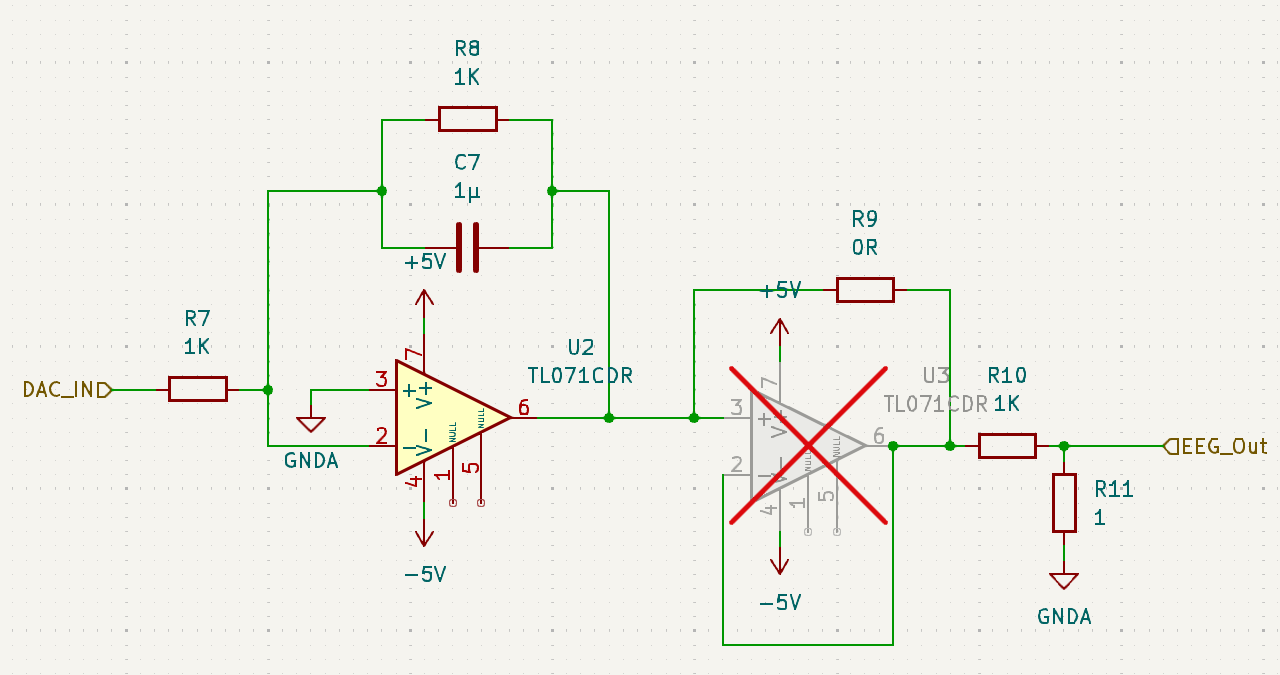
\includegraphics[width=0.8\textwidth]{bilder/Operationsverstaerker_Block.png}
    \caption{Operationsverstärker-Block der Platine}
    \label{fig:operationsverstaerker_block}
\end{figure}

Der Operationsverstärker-Block dient der analogen Nachbearbeitung der vom \gls{dac} bereitgestellten Ausgangssignale. Zum Einsatz kommt der TL071CDR, ein rauschoptimierter Operationsverstärker, der in dieser Anwendung als aktiver Tiefpassfilter erster Ordnung konfiguriert ist. Die Hauptfunktion besteht in der Glättung der Signale und der Unterdrückung hochfrequenter Störanteile.
Die Verstärkung des Filters ist auf 1 eingestellt, um die Signalform nicht zu verändern und gleichzeitig die Spannungsausgabe im gewünschten Millivolt-Bereich zu halten.
Optional kann ein zusätzlicher Operationsverstärker bestückt werden, der als Spannungsfolger (Buffer) wirkt. Dieser dient zur Reduzierung der Ausgangsimpedanz und kann insbesondere bei empfindlichen Messeingängen oder längeren Leitungswegen zur Verbesserung der Signalqualität beitragen. In der Standardkonfiguration ist dieser Pfad durch einen Jumper überbrückt und nicht bestückt.


\subsection{Spannungsversorgung}
\begin{figure}[H]
    \centering
    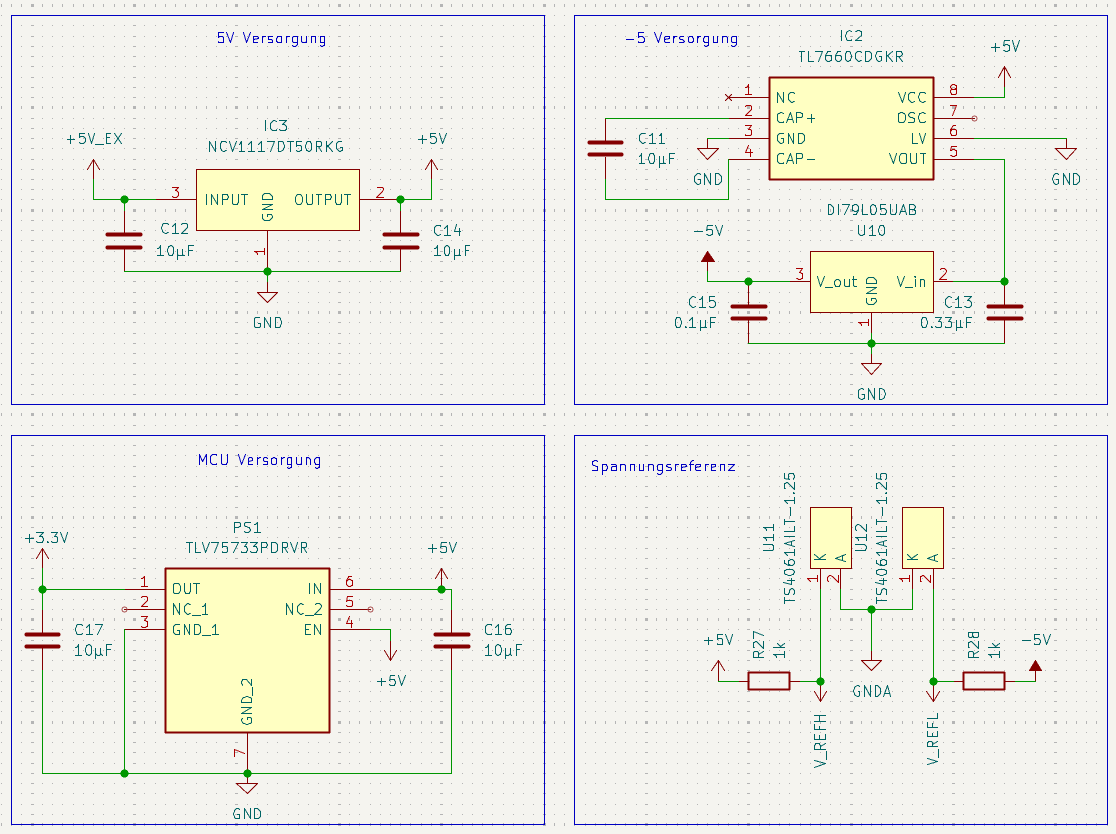
\includegraphics[width=0.8\textwidth]{bilder/Bipolar_Power.png}
    \caption{Spannungsversorgungsblock der Platine}
    \label{fig:spannungsversorgung}
\end{figure}

Die Spannungsversorgung der Platine erfolgt primär über eine USB-Schnittstelle, die eine Eingangsspannung von 5\,V bereitstellt. Diese Spannung wird durch den Linearregler NCV1117DT50RKG stabilisiert und zur Versorgung des DACs sowie der analogen Ausgangsstufen verwendet.
Für die Versorgung des Mikrocontrollers steht ein separater Low-Dropout-Regler (TLV75733PDRVR) zur Verfügung, der die benötigten 3{,}3\,V bereitstellt.
Da der \gls{dac} DAC8412FPZ eine symmetrische Versorgung von $\pm$5\,V erfordert, wird zusätzlich ein invertierender DC/DC-Wandler (LT3580EDD) eingesetzt. Dieser erzeugt aus der 5\,V-Versorgungsspannung eine negative Spannung von –5\,V, die ebenfalls zur Versorgung der Operationsverstärker verwendet wird.
Zudem benötigt der \gls{dac} eine präzise Referenzspannung. Diese wird über zwei Shunt-Referenzbausteine vom Typ TS4061AILT-1.25 realisiert und stellt eine stabile $\pm$1{,}25\,V-Referenz zur Verfügung. Diese Referenz ist entscheidend für die Genauigkeit der analogen Ausgangssignale.

\subsection{USB-Block}
\begin{figure}[H]
    \centering
    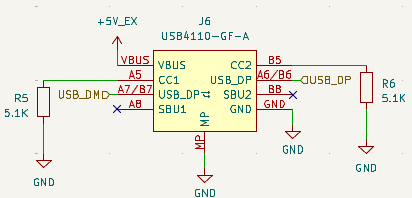
\includegraphics[width=0.8\textwidth]{bilder/USBC_Port.png}
    \caption{USB-Block der Platine}
    \label{fig:usb_block}
\end{figure}

Der USB-Block bildet die primäre Schnittstelle zur Stromversorgung der Platine. Über einen USB-C-Anschluss wird eine standardisierte 5\,V-Spannung bereitgestellt, die anschließend im Spannungsversorgungsblock weiter aufbereitet wird. Zusätzlich enthält der Block grundlegende Schutz- und Filterelemente zur Absicherung der Versorgungsspannung gegen Spannungsspitzen und Verpolung.
Optional kann die USB-Schnittstelle auch zur Datenübertragung mit dem Mikrocontroller verwendet werden, beispielsweise während der Programmierung oder zum Debugging über die serielle Schnittstelle. In der typischen Anwendung wird die Kommunikation jedoch vollständig über die WLAN-Funktion des ESP32 abgewickelt.

\section{Layout und PCB-Design}

\begin{figure}[H]
    \centering
    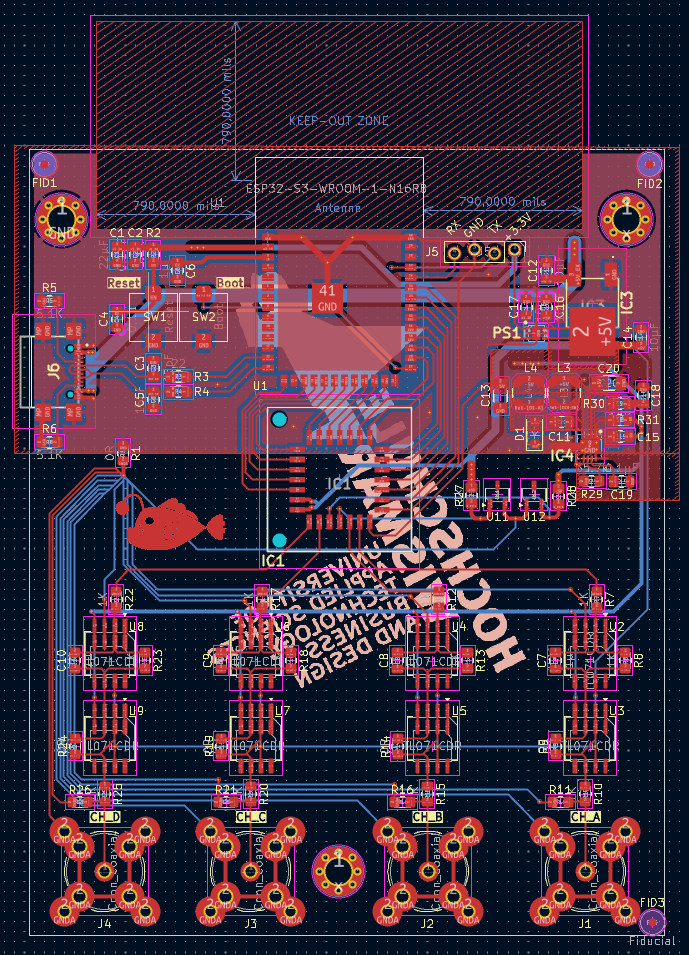
\includegraphics[width=0.8\textwidth]{bilder/Platinen-Layout.png}
    \caption{Layout der Platine}
    \label{fig:usb_block}
\end{figure}

Das PCB-Design wurde mit Fokus auf klare Signalführung, minimale Störanfälligkeit und eine strukturierte Blocktrennung umgesetzt. Die zweilagige Leiterplatte gliedert sich logisch in funktionale Bereiche, wobei sowohl die digitale Steuerung als auch die analogen Ausgangspfade übersichtlich und EMV-gerecht angeordnet sind.
Der Mikrocontroller (ESP32-S3) befindet sich im oberen Bereich der Platine und kommuniziert über eine parallele Busanbindung mit dem darunter angeordneten DAC8412FPZ. Die digitalen Steuersignale sind dabei als kurze, breit geführte Leitungen ausgeführt, um Reflexionen und Timing-Probleme zu minimieren.
Die vier analogen Ausgangskanäle befinden sich im unteren Bereich der Platine. Jeder Kanal verfügt über eine eigene Tiefpassfilterstufe sowie individuell geführte Ausgänge, die über identisch dimensionierte Leitungen auf korrekte Impedanz und Symmetrie geachtet wurden.
Die Versorgungsspannungen verlaufen sternförmig von der zentralen Spannungsaufbereitung aus, wobei Filterkondensatoren lokal an jedem Block platziert sind. Besonders im Bereich der symmetrischen Versorgung (±5\,V) und der Referenzspannungen wurde auf kurze Wege, Masseführung und Potentialtrennung geachtet.
Zudem wurde eine definierte „Keep-Out-Zone“ um die Antenne des ESP32 ausgewiesen, um Störungen im WLAN-Bereich zu vermeiden.


\begin{figure}[H]
    \centering
    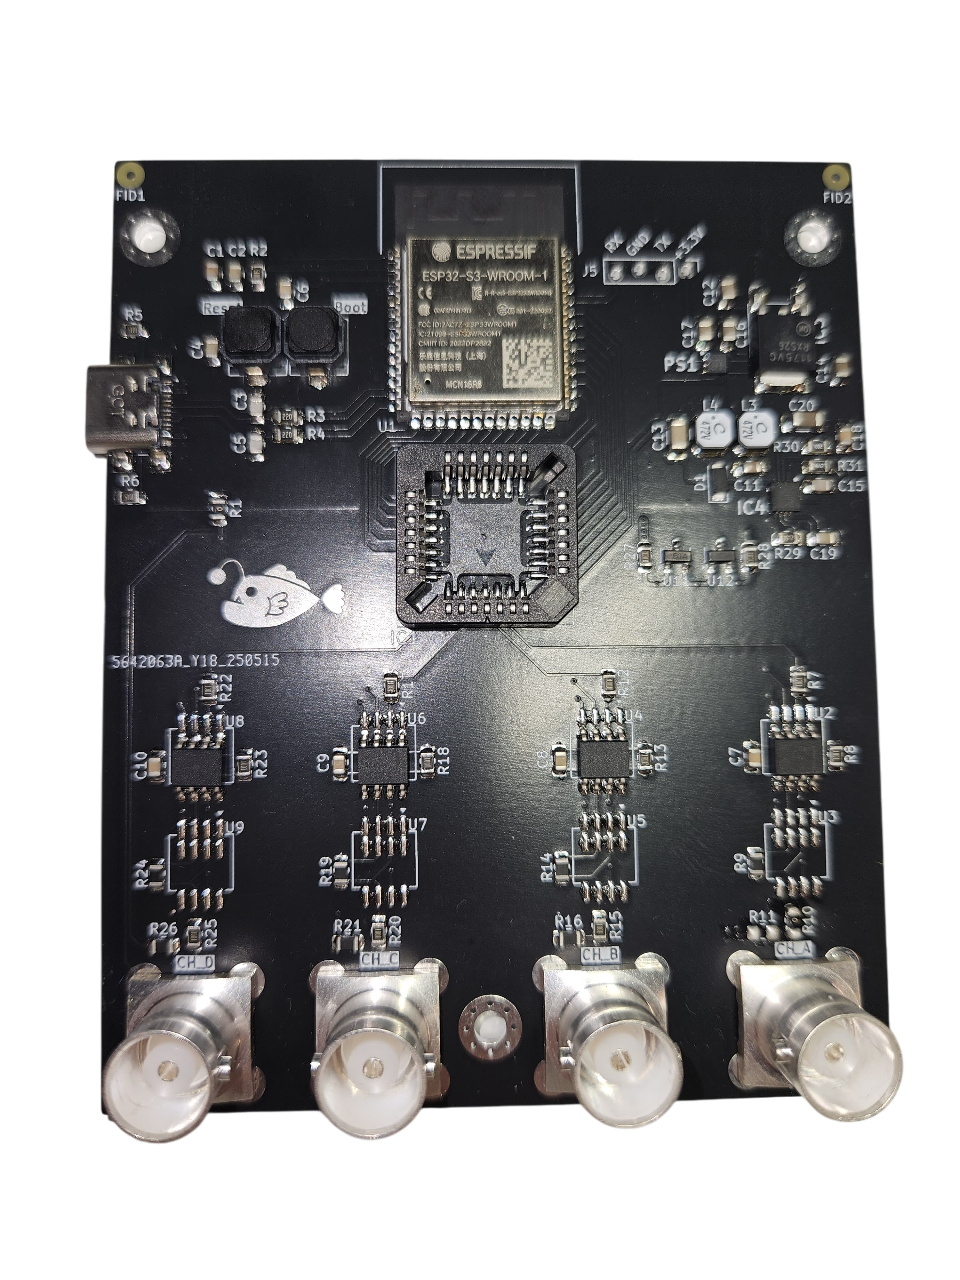
\includegraphics[width=0.7\textwidth]{bilder/Platine_bestueckt.png}
    \caption{Bestückte Platine}
    \label{fig:platine_bestueckt}
\end{figure}


% Schluss
\chapter{Zusammenfassung und Ausblick}
\label{schluss}

\section{Zusammenfassung}

Im Rahmen dieses Projekts wurde eine funktionsfähige Demonstrationsplatine zur Erzeugung synthetischer EEG-Signale entwickelt. Ziel war es, ein intuitiv bedienbares und technisch robustes Gerät für den Einsatz im Unterricht bereitzustellen. 

Die entwickelte Schaltung basiert auf einem ESP32-S3 Mikrocontroller in Kombination mit einem hochauflösenden DAC (DAC8412FPZ). Über vier unabhängige Ausgänge können benutzerdefinierte Signale analog ausgegeben und über Operationsverstärker geglättet werden. Die Parametrierung erfolgt über eine browserbasierte Weboberfläche, die vollständig ohne zusätzliche Softwareinstallation auskommt.

Während der Testphase zeigten sich einige Einschränkungen: Die vom invertierenden DC/DC-Wandler erzeugte negative Versorgungsspannung enthielt ein störendes hochfrequentes Signal. Dieses lässt sich jedoch durch einen nachgeschalteten Low-Dropout-Regler (LDO) wirksam unterdrücken. Alternativ wurde erfolgreich eine Versorgung über zwei symmetrisch verschaltete Lithium-Akkus getestet, wodurch die Störungen vollständig vermieden wurden.

Die Signalqualität im Mikrovoltbereich war zunächst stark von Rauschanteilen überlagert. Mittels spektraler Analyse (FFT) konnte das Nutzsignal jedoch nachgewiesen werden. Durch das Überbrücken des Spannungsteilers mittels 0-Ohm-Jumpern lässt sich das Signal alternativ auch im Millivoltbereich nutzen, was eine deutlich einfachere Auswertung per Oszilloskop ermöglicht.

\section{Ausblick}

Die derzeitige Version erfüllt alle grundlegenden Anforderungen an eine signalgebende EEG-Demoplatine. Dennoch ergeben sich mehrere sinnvolle Erweiterungs- und Optimierungsmöglichkeiten:

\begin{itemize}
  \item \textbf{Verbesserung der Filterung:} Der Einsatz eines höherwertigen analogen Tiefpassfilters (z.\,B. zweiter Ordnung oder Sallen-Key-Topologie) könnte die Rauschunterdrückung weiter verbessern. Dies muss jedoch experimentell verifiziert werden.
  \item \textbf{Stromversorgung:} Eine saubere Glättung der bipolare Versorgung über LDOs oder Versorgung mittels Akkus wäre langfristig stabiler als ein DC/DC-Wandler.
  \item \textbf{Signalbibliothek:} Eine optionale, nicht im Projekt enthaltene Sammlung vordefinierter Signalformen (z.,B. Alpha- oder Betawellen) könnte zukünftig über die Weboberfläche eingebunden werden.
  \item \textbf{Live-Visualisierung:} Eine grafische Darstellung der aktuellen DAC-Ausgabe direkt auf der Weboberfläche würde die Bedienung deutlich intuitiver gestalten. Dadurch könnten Nutzerinnen und Nutzer die Signalform in Echtzeit mitverfolgen, ohne auf externe Messgeräte wie ein Oszilloskop angewiesen zu sein.
\end{itemize}

Insgesamt bietet die entwickelte Platine eine solide Grundlage für den universitären Einsatz und stellt eine flexible Plattform für weitere didaktische und technische Weiterentwicklungen dar.


% =========
%  Anlagen
% =========

\begin{appendices}

  \chapter{Beispiele}\label{beispiel}

Beispielkapitel.
\lipsum[2]

\section{Ein Abschnitt}
Beispielabschnitt.

Aufzählungen werden mit der \code{enumerate} Umgebung erstellt:
\begin{enumerate}
  \item{Beispielpunkt A}
  \item{Beispielpunkt B}
  \item{\ldots}
\end{enumerate}

Sollen nur Stichpunkte abgebildet werden, so nimmt man dafür eine \code{itemize} Umgebung:
\begin{itemize}
  \item{Beispielpunkt C}
  \item{Beispielpunkt D}
  \item{\ldots}
\end{itemize}

\subsection{Ein Unterabschnitt}

Beispieltext.

\subsubsection{Ein Unter-Unterabschnitt}

Das ist die niedrigste Ebene.

\section{Tabellen}

Tabelle~\ref{tab:bsp} ist eine Beispieltabelle.
Man beachte die Position der Beschriftung.
\lipsum[1]

\begin{table}[!htbp]
  \caption{Beispieltabelle}\label{tab:bsp}
  \centering{%
    \begin{tabular}{|c|c|}
      \hline
      \textbf{Zeitpunkt (s)} & \textbf{Wert} \\
      \hlineB{3}
      0                      & 0.0           \\
      \hline
      1                      & 0.3           \\
      \hline
      2                      & 0.9           \\
      \hline
    \end{tabular}
  }
\end{table}

Ein wenig aufwendiger ist Tabelle \ref{tab:bsp2}.
\lipsum[3]

\begin{table}[!htbp]
  \caption{Tabelle mit \code{tabularx}, farbigen Zellen und Multicolumn.}
  \label{tab:bsp2}
  \centering {
    \sffamily
    \begin{tabularx}{0.3\textwidth}{|X|l|}
      \hline
      \rowcolor{gray!30!white}\multicolumn{2}{|c|}{\textbf{Schema} EAV} \\
      \hline
      \rowcolor{gray!30!white}\textbf{Spalte} & \textbf{Datentyp}       \\
      \hline
      \underline{id}                          & INTEGER                 \\
      \hline
      entität                                 & VARCHAR                 \\
      \hline
      attribut                                & VARCHAR                 \\
      \hline
      wert                                    & FLOAT                   \\
      \hline
    \end{tabularx}
  }
\end{table}

\section{Grafiken}

\lipsum[1]

\subsection{Rastergrafik}

Bild~\ref{fig:bsp} zeigt das Hochschullogo.
Es wird als JPEG-Datei eingebunden.
Man kann aber auch andere Formate wie PNG, EPS oder PDF auf diese Weise einbinden.

\begin{figure}[!htbp]
  \centering{%
    
\includegraphics[width=0.2\linewidth]{bilder/HSLogo.jpg}
    \caption{Logo der Hochschule Wismar}\label{fig:bsp}
  }
\end{figure}

\lipsum[2]

\subsection{In \LaTeX{} erzeugte Grafiken}

Bild~\ref{fig:tikzbsp} erzeugt eine Grafik mit dem Paket Ti\textit{k}Z\index{Ti\textit{k}Z}.

\begin{figure}[!htbp]
  \centering{%
    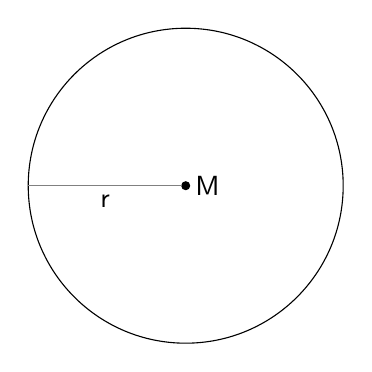
\begin{tikzpicture}
      \draw[black, thin] (0,0) circle (2);
      \filldraw[black] (0,0) circle (0.05) node[right] {\sffamily{M}};
      \draw[gray, thin] (-0.05,0) -- (-2,0) node[black, below, pos=0.5] {\sffamily{r}};
      \end{tikzpicture}
      \caption{Grafik mit Ti\textit{k}Z}\label{fig:tikzbsp}
  }
\end{figure}

So können beispielsweise auch Schaltpläne direkt im \LaTeX-Quelltext skizziert werden, wie Bild \ref{circuit} zeigt.

\begin{figure}[!htbp]
  \centering{%
    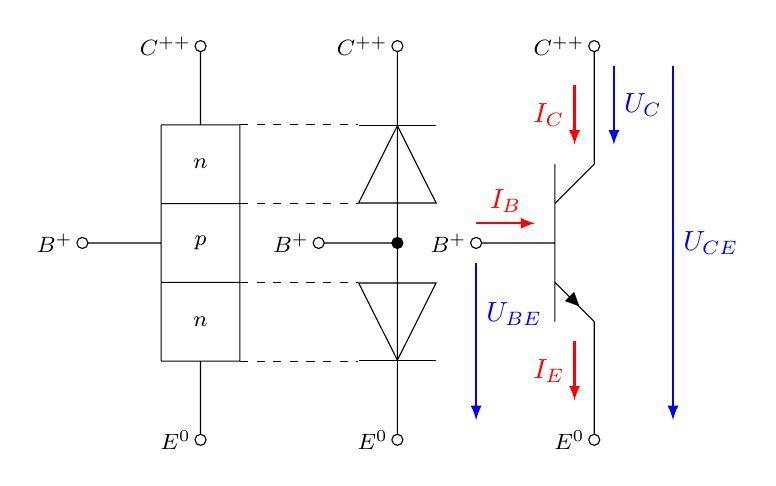
\begin{tikzpicture}[scale=0.5, circuit ee IEC, font=\sffamily\footnotesize]
      \tikzset{%
        Pfeil/.style={thick,shorten >=#1,shorten <=#1,->,>=latex},
        UPfeil/.style={blue,Pfeil=#1,font={\sffamily\itshape}},
        IPfeil/.style={red,Pfeil=#1,font={\ttfamily\itshape}}
      }

      \draw (0,0) -- (2,0)
      (3,3) -- (3,5)
      (3,-3) -- (3,-5)
      (2,-3) -- (2,3)
      (4,-3) -- (4,3)
      (2,3) -- (4,3)
      (2,-3) -- (4,-3)
      (2,1) -- (4,1)
      (2,-1) -- (4,-1)
      (8,-5) -- (8,5)
      (6,0) -- (8,0)
      (10,0) -- (12,0)
      (12,2) -- (12,-2)
      (13,2) -- (12,1)
      (13,-2) -- node [rotate=-45]{$\blacktriangleright$} (12,-1)
      (13,2) -- (13,5)
      (13,-2) -- (13,-5);

      \draw[fill=white] (0,0) circle (4pt) node [left] {$B^+$}
      (3,5) circle (4pt) node [left] {$C^{++}$}
      (3,-5) circle (4pt) node [left] {$E^0$}
      (6,0) circle (4pt) node [left] {$B^+$}
      (8,5) circle (4pt) node [left] {$C^{++}$}
      (8,-5) circle (4pt) node [left] {$E^0$}
      (10,0) circle (4pt) node [left] {$B^+$}
      (13,5) circle (4pt) node [left] {$C^{++}$}
      (13,-5) circle (4pt) node [left] {$E^0$};

      \draw[fill=black] (8,0) circle (4pt);

      \node [diode={circuit symbol size = width 8pt height 8pt}, point down] at (8,-2) {};
      \node [diode={circuit symbol size = width 8pt height 8pt}, point up] at (8,2) {};

      \draw[dashed] (4,3) -- (7,3)
      (4,1) -- (7,1)
      (4,-1) -- (7,-1)
      (4,-3) -- (7,-3);

      \node at (3,2) {$n$};
      \node at (3,0) {$p$};
      \node at (3,-2) {$n$};

      \draw[IPfeil=0em](12.5,-2.5) -- node [left]{$I_E$}(12.5,-4);
      \draw[IPfeil=0em](12.5,4) -- node [left]{$I_C$}(12.5,2.5);
      \draw[IPfeil=0em](10,0.5) -- node [above]{$I_B$}(11.5,0.5);
      \draw[UPfeil=0em](10,-0.5) -- node [right, yshift=1em]{$U_{BE}$}(10,-4.5);
      \draw[UPfeil=0em](13.5,4.5) -- node [right]{$U_C$}(13.5,2.5);
      \draw[UPfeil=0em](15,4.5) -- node [right]{$U_{CE}$}(15,-4.5);
    \end{tikzpicture}
    \caption{Beispiel für einen Schaltplan mit Ti\textit{k}Z}
    \label{circuit}
  }
\end{figure}

Das Paket \code{smartdiagram} bietet darüber hinaus auch Funktionen zur automatischen Erzeugung spezieller Grafiken (siehe Bild \ref{fig:smart}).
Mehr dazu in der entsprechenden Dokumentation \cite{smart}.

\begin{figure}[!htbp]
  \centering{\smartdiagram[sequence diagram]{Rühren,Kneten,Backen}}
  \caption{Sequenzdiagramm mit dem \code{smartdiagram} Paket}
  \label{fig:smart}
\end{figure}

Natürlich können Plots und andere Grafiken in den Programmen der Wahl erstellt und dann als Bilddatei mit einem \verb$\includegraphics$ eingebunden werden.
Allerdings ist auch dies in \LaTeX{} direkt möglich, wie Bild \ref{fig:plot} zeigt\index{Plot}.

\begin{figure}[!htbp]
  \center {
    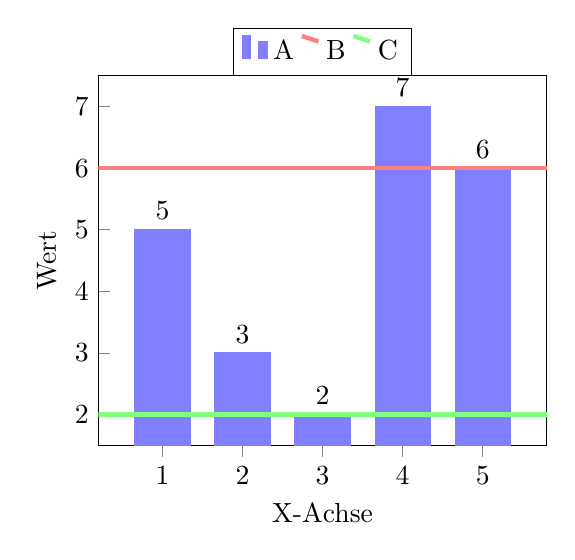
\begin{tikzpicture}
      \begin{axis}[
          xtick=data,
          ytick={0, 1, 2, 3, 4, 5, 6, 7, 8},
          x tick label style={/pgf/number format/1000 sep=},
          xlabel=X-Achse,
          ylabel=Wert,
          ytick distance=2,
          xtick pos=left,
          ytick pos=left,
          enlarge x limits=0.2,
          enlarge y limits=0.1,
          legend style={at={(0.5,1.13)},anchor=north,legend columns=-1},
          ybar,
          bar width=.7cm,
          width=0.6\textwidth,
        ]
        \addplot[
          draw=blue!50!white,
          fill=blue!50!white,
          nodes near coords,
          nodes near coords align={vertical},
        ]coordinates {(1,5) (2,3) (3,2) (4,7) (5,6)};

        \addplot[
          draw=red!50!white,
          sharp plot,
          ultra thick,
          update limits=false
        ]coordinates {(0,6) (6,6)};

        \addplot[
          draw=green!50!white,
          sharp plot,
          ultra thick,
          update limits=false
        ]coordinates {(0,2) (6,2)};

        \legend{A, B, C}

      \end{axis}
    \end{tikzpicture}
  }
  \caption{Ein Balkendiagramm}
  \label{fig:plot}
\end{figure}

\section{Quellcode-Listings}

Minted lässt inline Code wie z.B. \mintinline[style=vs]{c}{print("Hallo, LaTeX!")} zu.

Für Listings können Dateien zum Einbinden angegeben werden (Listing \ref{lst:example-file}).

\begin{listing}[!htbp]
  \inputminted{c}{./anlagen/exampleCode.c}
  \caption{C-Quelltext aus Datei}
  \label{lst:example-file}
\end{listing}

Alternativ kann der Quelltext direkt in eine \code{minted} Umgebung eingefügt werden (Listing \ref{lst:example-intext}).

\begin{listing}[!htbp]
  \begin{minted}{c}
    #include <stdio.h>

    int main(void)
    {
      printf("Hallo nochmal!\n");

      return 0;
    }
  \end{minted}
  \caption{Weiteres Beispiel für C-Quelltext}
  \label{lst:example-intext}
\end{listing}

Beide Beispiele werden im voreingestellten Stil dargestellt.
Das Paket \code{minted} bietet weitere Farbschemata, wie das Beispiel \ref{lst:example-color} zeigt.
In der Präambel des Dokuments kann mit \mintinline{tex}{\setminted{style=...}} der globale Stil der Listings angepasst werden.

\begin{listing}[!htbp]
  \renewcommand\theFancyVerbLine{%
    \rmfamily
    \textcolor[rgb]{0.7,0.7,0.7}{\tiny {\arabic{FancyVerbLine}}}%
  }
  \begin{minted}[style=solarized-dark, bgcolor=solarized@base03]{cpp}
    #include <iostream>

    int main(void)
    {
      std::cout << "Hallo (diesmal in Farbe)!" << std::endl;

      return 0;
    }
  \end{minted}
  \caption{C++ Quelltext im \textit{Solarized} Farbschema}
  \label{lst:example-color}
\end{listing}

Eine Auswahl von bereits definierten Styles ist auf der Webseite von Pygments (\url{https://pygments.org/styles/}) zu finden.

\textbf{Aber Achtung:} Die Zeilennummerierung ist standardmäßig schwarz und kann nur durch das Überschreiben von \textit{\textbackslash theFancyVerbLine} geändert werden.
Dies kann global in der Präambel (siehe \code{renewcommand...} in Listing \ref{lst:example-color}) für alle Listings geschehen oder lokal (ebenfalls Listing \ref{lst:example-color}) in der \code{listing} Umgebung.

\section{Eine Formel}

Beispiel für Formeln. Sollen Formeln linksbündig dargestellt werden, dann in der Datei \textit{header.tex} die Option \code{fleqn} entkommentieren (Option der Dokumentenklasse)\index{Formel}.

\begin{equation}
  c = \sqrt{a^2 + b^2}
\end{equation}

Im Math-Mode kann man zwar griechische Buchstaben schreiben, aber im normalen Modus nicht ohne das Paket \code{textgreek}. Aus \verb$\textmu$ wird so zum Beispiel ein \textmu.

\section{Algorithmen}

\begin{algorithm}[htb]
  \begin{algorithmic}[1]
    \REQUIRE $\Gamma$: ein Parameter \\ $M$: noch ein Parameter  \\  $m$: und noch ein Parameter \\ $k$: letzter Parameter
    \ENSURE $B = \{b_i|i = 1, 2,\dots, m\}$ ist das angestrebte Ergebnis
    \STATE Eine simple Angabe, die auch Formeln zulässt: $k$ \leftarrow $\{r_i \in \mathbb{R}^M |i = 1, 2,\dots, m\}$
    \IF{eine Zustand zutrifft}
    \STATE tue Etwas
    \ELSIF{eine Zustand zutrifft}
    \STATE tue etwas Anderes
    \ELSE
    \STATE führe die Standardaktion aus
    \ENDIF
    \FOR{$i=0$ \TO $10$}
    \STATE tue Etwas
    \ENDFOR
    \WHILE{eine Zustand zutrifft}
    \STATE tue Etwas
    \ENDWHILE
    \REPEAT
    \STATE tue Etwas
    \UNTIL{eine Zustand zutrifft}
    \LOOP
    \STATE tue Etwas
    \ENDLOOP
    \RETURN $(x+y)/2$ \COMMENT eine Anmerkung
  \end{algorithmic}
  \caption{Beispiel für einen Algorithmus}
  \label{alg:example}
\end{algorithm}

\section{Referenzen}
\label{refn}

In Kapitel \ref{beispiel} auf Seite \pageref{refn} finden Sie einige Beispiele dafür, wie Referenzen in \LaTeX~funktionieren.

\subsection{Abkürzungen}

Eine weit verbreitete Architektur für Web-Anwendungen ist der \gls{lamp}-Stack (Beispiel für die Nutzung eines Akronyms).
Wird das gleiche Akronym nochmals verwendet, wird automatisch die Kurzform \gls{lamp}-Stack verwendet.
Pluralformen sind ebenfalls automatisiert möglich, so wird aus dem \gls{qrc} im Plural die \glspl{qrc}.
Außerdem ist es möglich die volle Form, wie beim ersten Benutzen (\acrfull{qrc}), oder nur die ausgeschriebene Form (\acrlong{qrc}) zu wiederholen.

\subsection{Glossar}

MongoDB ist ein Datenbanksystem, das in die Kategorie der \gls{nosql}-Datenbanken fällt (Beispiel für einen Eintrag ins Glossar).
Manchmal wird eine Mischung aus Glossareintrag und Akronym benötigt, zum Beispiel um einen eigentlich geläufigen Fachbegriff wie \gls{dos} zu erklären.

\subsection{Symbolverzeichnis}

\begin{equation}
  \alpha = \frac{1}{e} + sin(\phi)
\end{equation}

Hier die Symbole \gls{symb:phi} und \gls{symb:e}, welche im Symbolverzeichnis erscheinen, um ihre Bedeutung zu erklären.

\subsection{Literatur}

Und natürlich kann auch auf Literatur verwiesen werden.
Alle Quellen werden in diesem Beispiel in die Datei \textit{quellen.bib} geschrieben.
In \citetitle{unterstein12} \cite{unterstein12} geht es beispielsweise um Datenbanken.
Der Artikel von \citeauthor{goldberg91} \cite{goldberg91} ist auch ganz interessant.
Zum Schluss noch eine online Quelle \cite{wave} und eine lange URL \cite{long}, die im \nameref{bib} hoffentlich ordentlich auf mehrere Zeilen aufgeteilt wird.

% \section{Ligaturtest}

% \begin{description}
%   \item[Ligaturen erlaubt]{Affe, flink, offiziell}
%   \item[Ligaturen verboten]{Kaufleute, Ablauffolge, Stoffjacke}
% \end{description}


\end{appendices}

% ===============
%  Verzeichnisse
% ===============

% Verzeichnisse mit einzeiligem Zeilenabstand
\singlespacing

% Literaturverzeichnis
\listofreferences

% Abbildungsverzeichnis einfügen
\listoffigures

% Tabellenverzeichnis einfügen
\listoftables

% Algorithmenverzeichnis einfügen
\listofalgorithms

% % Quelltextverzeichnis einfügen
\listoflistings

% Abkürzungsverzeichnis
\listofacronyms

% Symbolverzeichnis
\listofsymbols

% falls ein anderer Glossar-Stil genutzt wird und die zweite Spalte zu schmal ist:
% \setlength{\glsdescwidth}{0.8\linewidth}

% Glossar einfügen
\printglossary

% Index einfügen
\printindex

% wieder auf 1½-fachen Zeilenabstand umschalten
\normalspacing

% =========================================
%  Selbstständigkeitserklärung, CD, Thesen
% =========================================

% Selbstständigkeitserklärung
\makedeclarationofindependence



% Thesen (allerletzte Seite); Thesen bitte immer durch Semikolons trennen
\maketheses{%
  These 1;
  These 2;
  \ldots
}

\end{document}

% =============
%  Ende Thesis
% =============
